\documentclass[conference]{IEEEtran}
\IEEEoverridecommandlockouts

\usepackage{amsmath,amsfonts,amssymb}
\usepackage{graphicx}
\usepackage{booktabs}
\usepackage{array}
\usepackage{multirow}
\usepackage{url}
\usepackage[skip=4pt]{caption}
\usepackage{placeins}
\usepackage{balance}
\usepackage{tikz}
\usetikzlibrary{shapes.geometric, arrows, positioning, fit, calc}
\usepackage{algorithm}
\usepackage{algpseudocode}
\usepackage{xcolor}
\usepackage[hidelinks]{hyperref}

\setlength{\textfloatsep}{6pt}
\setlength{\floatsep}{6pt}
\setlength{\intextsep}{6pt}

\title{An Appraisal-Augmented Dueling Double DQN with a Bootstrap Ensemble for
Cognitively Grounded Affective Modelling in Reinforcement Learning Agents}

\author{
\IEEEauthorblockN{Dev Shrut Jain}
\IEEEauthorblockA{Department of Artificial Intelligence \\
SVNIT, Surat \\
Email: jaindevshrut@gmail.com}
\and
\IEEEauthorblockN{Sweta Rana}
\IEEEauthorblockA{Department of Artificial Intelligence \\
SVNIT, Surat \\
Email: ranasweta2005@gmail.com}
\and
\IEEEauthorblockN{Krish Rathod}
\IEEEauthorblockA{Department of Artificial Intelligence \\
SVNIT, Surat \\
Email: krishrathod5696@gmail.com}

}

\begin{document}

\maketitle

\begin{abstract}
Scherer's Component Process Model treats emotion as the outcome of a sequence
of cognitive evaluations of goal-relevant events. A recent line of work
operationalises these evaluations inside a reinforcement learning (RL) loop,
reading appraisal directly from quantities the agent already maintains:
transition counts, the temporal-difference (TD) error, and the range of action
values. The drawback is structural. Three of the four checks in the reference
scheme depend on the TD error, so a fourth of the dimensionality carries the
same shared signal, and emotions that differ on something other than TD
magnitude collapse onto each other. We address that bottleneck with two
coupled changes. The actor-critic backbone is replaced with a Dueling Double
DQN that carries a bootstrap ensemble of $K{=}3$ value heads, which makes
$V(s)$, the centred advantage, and an across-head dispersion available as
named outputs. The four-dimensional appraisal vector is then extended to
eight dimensions by adding four channels designed to read disjoint
statistics: \emph{predictability} from the ensemble dispersion,
\emph{anticipation} from the dueling $V$-head, \emph{urgency} from the
within-episode time index, and \emph{familiarity} from log-scaled state-visit
counts. The agent is trained for 60{,}000 frames on a $7{\times}7$
key-and-lava grid world; appraisal vectors are then mapped to four
task-event proxies (neutral, joy, satisfaction, despair) by a multinomial
logistic regression. Under identical seed and backbone, the extended vector
nearly doubles the effective rank of the appraisal covariance
($1.58{\to}3.18$), raises classification accuracy from $64.8\%$ to $90.3\%$,
lifts $R^{2}$ from $0.366$ to $0.757$, and reduces RMSE from $0.345$ to
$0.214$, with no change to greedy-policy return. A permutation-importance
analysis attributes the gain to the new dimensions: four of the five most
discriminative channels are the ones we introduce. We do not paper over the
single residual redundancy---\emph{anticipation} reaches a variance-inflation
factor of $7.4$ once the dueling head converges, and we explain why it
is structural rather than a modelling oversight. As a
parallel comparison, we also build a Quantile-Regression DQN backbone
(Method~2b) following~\cite{dabney2018qrdqn}, in which the dueling V-head and
the bootstrap ensemble are replaced by a $51$-atom return distribution and
the appraisal vector reads its uncertainty signal from intra-distribution
spread; we report its numbers honestly alongside the headline configuration
so that the design trade-off is visible to the reader. Two preliminary
configurations explored along the way---Method~1a (a vanilla DQN with a
six-dimensional appraisal vector and a ten-head MLP ensemble) and
Method~2a (a $64$-quantile distributional value head with a calibrated
SVM classifier on a four-dimensional Scherer mapping)---are documented
in full with the empirical evidence that motivated their replacement
by Method~1b and Method~2b respectively. We end with concrete
pointers toward a vignette-grounded extension.
\end{abstract}

\begin{IEEEkeywords}
Affective computing, reinforcement learning, appraisal theory, Dueling DQN,
bootstrap ensemble, epistemic uncertainty, computational emotion modelling.
\end{IEEEkeywords}

\section{Introduction}
\label{sec:intro}

Emotions are not a layer painted on top of human cognition; they are
woven into how attention is allocated, how candidate actions are weighed,
and how learning is biased toward salient outcomes. Building artificial
agents that can produce and read such signals has been a long-running aim
of affective computing, in part because agents that can do both interact
more naturally with the people they serve~\cite{picard1997affective,marsella2009ema}.

One way to build that machinery is to bolt an emotion module onto a
policy. A more economical alternative falls out of the appraisal
literature: Scherer's Component Process Model (CPM) describes emotion as
the cumulative output of a hierarchy of cognitive
checks~\cite{scherer2001appraisal,scherer2009dynamic}, and most of those
checks happen to read quantities that an RL agent already maintains.
Under this lens, emotion and goal-directed action share machinery rather
than competing for it.

The clearest computational expression of this view is the recent work of
Zhang, Broekens and Jokinen~\cite{zhang2023modeling}, who place four CPM
checks (\emph{suddenness}, \emph{goal relevance}, \emph{conduciveness}
and \emph{power}) directly on top of a tabular Q-learning agent. Each
check is read from a quantity the algorithm already computes: transition
counts, the temporal-difference (TD) error, and the spread of
$Q(s,\cdot)$. The resulting four-dimensional vector is mapped to modal
emotions through a Support Vector Machine trained on theoretical Scherer
distributions, then validated against ratings from a vignette study.

\subsection{Motivation and Problem Statement}
The scheme of~\cite{zhang2023modeling} establishes that appraisal is
computationally extractable from RL signals. Two limitations show up
when one tries to scale or sharpen it.

\textbf{(L1) Information bottleneck.} Three of the four checks, namely
goal relevance, conduciveness, and (more weakly) power, are functions of the
TD error. A vector whose channels share a single source cannot, by
construction, distinguish emotions that differ on something else.
Boredom and a quiet neutral state are a useful test case: both produce
near-zero TD, both produce no surprise, and the only thing that
separates them is how familiar the agent is with the state. In a
TD-driven feature space they collapse together.

\textbf{(L2) Backbone-induced opacity.} The original work runs on a
tabular Q-table; the obvious deep generalisation is an A2C or PPO
actor-critic. Neither exposes $V(s)$ as a named output, and neither
produces a structured estimate of how confident the agent is in its own
values. Yet two appraisal-relevant signals, the absolute value level
and the epistemic disagreement among value estimates, live precisely
there. Reading them off indirectly is possible but introduces bias the
appraisal vector inherits.

Stated as a single question: can the cognitive expressiveness of an
RL-based appraisal vector be increased without trading away the agent's
task return or the mechanistic transparency of the appraisal formulas,
and can the gain be attributed to genuinely independent information
rather than to representational redundancy?

\subsection{Research Gap}
Earlier attempts to enrich appraisal-RL representations have mostly added
new RL machinery (distributional value learning, latent-variable
critics) without checking whether the new features carry information
that is \emph{statistically distinct} from the old ones. The vector
grows in length but not in informativeness, and decorrelation
diagnostics are rarely reported. Our remit is the inverse: treat
decorrelation as a design constraint up front. Every new dimension must
be computable from a statistic that is algebraically disjoint from those
already used, and the resulting orthogonality is then verified
empirically with a Pearson correlation matrix, per-dimension
variance-inflation factors, and the effective rank of the appraisal
covariance.

\subsection{Objectives and Contributions}
The contributions of this paper are four:
\begin{itemize}
\item A Dueling Double DQN with a bootstrap ensemble of $K$ value heads
serves as the appraisal substrate. The dueling split makes $V(s)$ and
the centred advantage available as separate named quantities; the
ensemble adds an epistemic-uncertainty signal that no prior backbone
exposes.

\item Four new channels extend the appraisal vector
of~\cite{zhang2023modeling} from four dimensions to eight:
\emph{predictability} (from ensemble dispersion), \emph{anticipation}
(from the dueling $V$-head), \emph{urgency} (from the within-episode
time index), and \emph{familiarity} (from log-scaled state-visit
counts). Each is read from a statistic that does not appear in the
original four formulas.

\item A full decorrelation audit accompanies the new vector: Pearson
correlation matrix, per-dimension VIF, and effective rank of the
appraisal covariance. Effective rank approximately doubles
($1.58{\to}3.18$), and four of the top five most discriminative
dimensions in a permutation-importance analysis turn out to be the
newly added ones.

\item A 60k-frame benchmark on a key-and-lava grid world, fully
reproducible from the artefacts archived under \texttt{runs/}, anchors
the empirical claims. Classification accuracy lifts from $64.8\%$ to
$90.3\%$; paper-style $R^{2}$ rises from $0.366$ to $0.757$; greedy
return is unchanged.

\item A transparent record of the two preliminary configurations
considered before settling on the headline pairing. Method~1a
(Section~\ref{sec:method1a}, a vanilla DQN with a six-dimensional
appraisal vector and an MLP ensemble) and Method~2a
(Section~\ref{sec:method2a}, a $64$-quantile distributional value head
with a calibrated SVM on a four-dimensional Scherer mapping) are
reported in full, with the empirical evidence that motivated their
replacement by Method~1b and Method~2b. The aim is to make the design
trajectory of the paper, not just its endpoint, auditable.
\end{itemize}

The remainder of the paper is organised as follows.
Section~\ref{sec:related} surveys the related literature.
Section~\ref{sec:background} reviews the necessary background on RL, dueling
networks and the CPM. Section~\ref{sec:method} develops the proposed
methodology, with mathematical formulations consolidated in
Section~\ref{sec:math}. Section~\ref{sec:impl} reports the implementation
details and Section~\ref{sec:experiments} the experimental protocol.
Sections~\ref{sec:results} and~\ref{sec:discussion} present and interpret the
results. Sections~\ref{sec:conclusion} and~\ref{sec:future} conclude and
outline the future scope.

\section{Related Work}
\label{sec:related}

\subsection{Cognitive and Computational Models of Emotion}
The cognitive turn in emotion research is generally traced to Lazarus's
appraisal theory~\cite{lazarus1991emotion}, which characterises emotion as the
output of an evaluative process applied to events with respect to an
individual's wellbeing. Scherer's Component Process Model (CPM) decomposes this
evaluation into a hierarchy of cognitive checks (relevance, implication,
coping potential and normative significance) that proceed in a partially
ordered sequence~\cite{scherer2001appraisal}. The OCC model of Ortony, Clore
and Collins~\cite{ortony1990cognitive} is closely related and remains widely
used for rule-based affect generation in agent architectures, while the
Emotion-and-Adaptation (EMA) model~\cite{marsella2009ema} provides a
process-level reinterpretation. These models share a commitment to emotion as
an information-processing phenomenon but differ in the level of operational
specificity they offer to a computational implementation.

\subsection{Reinforcement Learning Foundations}
Modern reinforcement learning rests on the Markov Decision Process (MDP)
formulation~\cite{sutton2018reinforcement}. Tabular methods such as
Q-learning~\cite{watkins1992qlearning} converge under suitable assumptions but
do not scale to high-dimensional observations. The Deep Q-Network of Mnih
\textit{et al.}~\cite{mnih2015human} demonstrated that experience replay, a
target network and a convolutional value approximator together yield
human-level performance on the Atari benchmark. Subsequent refinements that are
directly relevant to the present work include the Double DQN
correction~\cite{vanhasselt2016double} for value over-estimation, the dueling
architecture~\cite{wang2016dueling} for separating state-value from advantage,
and prioritised experience replay~\cite{schaul2016prioritized} for
TD-magnitude-weighted sampling. Bootstrapped
DQN~\cite{osband2016deepexploration} introduced the use of an ensemble of
randomly initialised value heads as a practical mechanism for deep exploration
through Thompson-style posterior sampling; we adapt the same construction here
for a different purpose, namely as a source of epistemic uncertainty for the
appraisal vector. Distributional RL, including the categorical
formulation of~\cite{bellemare2017distributional} and the
quantile-regression variant of~\cite{dabney2018qrdqn}, provides a
complementary mechanism for modelling return uncertainty but consumes
the appraisal layer with a distribution-valued signal whose projection
onto interpretable scalars introduces information loss; we examine this
trade-off empirically by building a parallel QR-DQN backbone (Method~2b,
Section~\ref{sec:method2b}) and comparing it head-to-head with our
headline configuration in Section~\ref{sec:method2_results}.

\subsection{Coupling Appraisal with Reinforcement Learning}
Several authors have argued that RL is a natural substrate for appraisal,
since both frameworks treat behaviour as goal-directed adaptation under
reward feedback~\cite{moerland2018emotion,broekens2007cognitive}. The recent
formulation of Zhang \textit{et al.}~\cite{zhang2023modeling}
is the closest antecedent to the present work and provides the four-check
appraisal scheme on which we build. Their model trains a tabular Q-learning
agent on small hand-designed MDPs that mirror vignette-based stimuli used in
human studies, then maps the resulting four-dimensional appraisal vector to
modal-emotion intensities through an SVM. The present paper retains the
operational mapping between RL signals and Scherer's checks but addresses two
limitations identified above through a deeper backbone and a richer feature
vector.

\subsection{Position of This Work}
The contribution we make sits at neither end of this literature. It is
not a new RL algorithm and it is not a new theory of emotion. It is a
change at the \emph{interface}: keep the appraisal-to-emotion mapping
roughly the way the literature has it (a discriminative classifier on a
fixed-length appraisal vector, no new emotion categories), but rework
the backbone so that more of the RL agent's internal state surfaces as
named quantities, and rework the appraisal vector so that those
newly-exposed quantities are actually consumed by channels designed to
be statistically independent of one another.

\section{Background and Theoretical Foundations}
\label{sec:background}

\subsection{Markov Decision Processes and Q-learning}
A finite Markov Decision Process is a tuple $\mathcal{M} = (S, A, P, R, \gamma)$
where $S$ is the state set, $A$ the action set,
$P : S \times A \times S \to [0, 1]$ the transition kernel, $R : S \times A
\to \mathbb{R}$ the reward function, and $\gamma \in [0, 1)$ the discount
factor. The action-value function under a policy $\pi$ is
$Q^{\pi}(s, a) = \mathbb{E}_{\pi}[\sum_{t=0}^{\infty} \gamma^{t} r_{t} \mid
s_{0}{=}s,\, a_{0}{=}a]$. Q-learning estimates $Q^{*}$ with the off-policy
update
\begin{equation}
Q(s, a) \leftarrow Q(s, a) + \alpha \big[ r + \gamma \max_{a'} Q(s', a') - Q(s, a) \big].
\label{eq:qlearn}
\end{equation}
The bracketed quantity is the temporal-difference error
\begin{equation}
\delta = r + \gamma \max_{a'} Q(s', a') - Q(s, a).
\label{eq:td}
\end{equation}

\subsection{Deep Q-Networks}
Deep Q-Networks~\cite{mnih2015human} approximate $Q$ with a parametric function
$Q_{\theta}$ trained by minimising the squared TD error against a slowly
updated target network $Q_{\theta^{-}}$:
\begin{equation}
\mathcal{L}(\theta) =
\mathbb{E}_{(s, a, r, s') \sim \mathcal{D}}
\Big[ \big( Q_{\theta}(s, a) - y \big)^{2} \Big],
\end{equation}
\begin{equation}
y = r + \gamma \max_{a'} Q_{\theta^{-}}(s', a').
\end{equation}
\textit{Double} DQN~\cite{vanhasselt2016double} replaces this target with
\begin{equation}
y_{\mathrm{DDQN}} = r + \gamma\, Q_{\theta^{-}}\!\big(s',\, \arg\max_{a'} Q_{\theta}(s', a')\big),
\end{equation}
which decouples action selection from action evaluation and reduces the
positive bias inherent in the $\max$ operator.

\subsection{Dueling Architecture}
The dueling architecture~\cite{wang2016dueling} factorises the value head as
\begin{equation}
Q_{\theta}(s, a) = V_{\theta}(s) + \Big( A_{\theta}(s, a) - \tfrac{1}{|A|} \sum_{a'} A_{\theta}(s, a') \Big),
\label{eq:dueling}
\end{equation}
which exposes the state-value $V(s)$ and the centred advantage $A(s, a) -
\overline{A}(s, \cdot)$ as separate quantities. This decomposition is critical
for the present work because it identifies, by construction, the two
appraisal-relevant signals embedded inside an otherwise opaque scalar:
$V(s)$ is the absolute value level (used by \emph{anticipation}) and the
centred advantage is the action-effect spread (used by \emph{power}).

\subsection{Bootstrap Ensembles and Epistemic Uncertainty}
A bootstrap ensemble~\cite{osband2016deepexploration} maintains $K$ value heads
$\{Q^{(k)}\}_{k=1}^{K}$ that share a feature trunk but are randomly initialised
independently. Disagreement among heads after training, quantified by the
per-state action-averaged standard deviation
\begin{equation}
\sigma_{K}(s) = \frac{1}{|A|} \sum_{a} \mathrm{std}_{k}\big(Q^{(k)}(s, a)\big),
\label{eq:qstd}
\end{equation}
provides an estimate of the agent's own \emph{epistemic} uncertainty about the
value of a state. We use this signal as the basis of the \emph{predictability}
appraisal.

\subsection{Component Process Model}
The CPM~\cite{scherer2001appraisal} treats emotion as the cumulative
output of a sequence of cognitive checks. The four checks
formalised by~\cite{zhang2023modeling}, namely suddenness, goal relevance,
conduciveness, and power, separate a useful subset of modal emotions
but cannot, on their own, tell apart emotions whose distinguishing
feature lies elsewhere: uncertainty (anxiety vs.\ determined anger),
absolute prospect (hope vs.\ realised joy), temporal pressure (panic
vs.\ despair), or familiarity (boredom vs.\ neutral). The four
dimensions we add are aimed at exactly those distinctions.

\section{Proposed Methodology}
\label{sec:method}

\subsection{System Overview}
Figure~\ref{fig:pipeline} summarises the overall pipeline. The agent observes
the environment state, selects an action through an $\varepsilon$-greedy
policy over the mean of the $K$ ensemble heads, receives a reward and a
successor state, and writes the transition into a prioritised replay buffer.
At every environment step the appraisal extractor reads (i)~the per-action
$Q$ values, (ii)~the dueling $V(s)$, (iii)~the across-head standard deviation
$\sigma_{K}$ and (iv)~the count tables maintained over visited states and
observed transitions, and emits an appraisal vector
$\mathbf{x}(s_{t}, a_{t}, s_{t+1}) \in \mathbb{R}^{8}$. After training, the
collected appraisal vectors and their event labels are passed to a
logistic-regression classifier that estimates emotion-class probabilities.

\begin{figure}[!t]
\centering
\resizebox{0.95\columnwidth}{!}{%
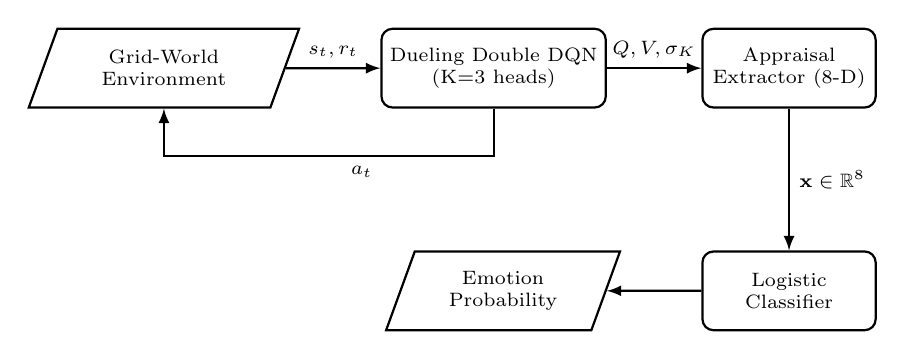
\begin{tikzpicture}[
  node distance=14mm and 12mm,
  every node/.style={font=\scriptsize},
  block/.style={rectangle, draw, thick, rounded corners,
                minimum width=22mm, minimum height=10mm,
                align=center, inner sep=3pt},
  io/.style={trapezium, draw, thick, trapezium left angle=70,
             trapezium right angle=110, minimum width=18mm,
             minimum height=10mm, align=center, inner sep=3pt},
  arrow/.style={-latex, thick}
]
% top row
\node[io]                                  (env)   {Grid-World\\Environment};
\node[block, right=of env]                 (agent) {Dueling Double DQN\\(K=3 heads)};
\node[block, right=of agent]               (extr)  {Appraisal\\Extractor (8-D)};
% bottom row
\node[block, below=18mm of extr]           (clf)   {Logistic\\Classifier};
\node[io,    left=of clf]                  (emo)   {Emotion\\Probability};

\draw[arrow] (env)   -- node[above, midway]{$s_t,r_t$} (agent);
\draw[arrow] (agent) -- node[above, midway]{$Q,V,\sigma_K$} (extr);
\draw[arrow] (extr)  -- node[right, midway]{$\mathbf{x}\in\mathbb{R}^{8}$} (clf);
\draw[arrow] (clf)   -- (emo);
% feedback action arrow underneath
\draw[arrow] (agent.south) -- ++(0,-6mm) -| (env.south)
              node[pos=0.2, below]{$a_t$};
\end{tikzpicture}%
}
\caption{End-to-end pipeline. The dueling Double DQN exposes
$Q$, $V$ and the cross-head standard deviation $\sigma_K$, all of
which are consumed by the eight-dimensional appraisal extractor.}
\label{fig:pipeline}
\end{figure}

\subsection{Environment Formulation}
We use a deterministic $7{\times}7$ grid world with a single key, three lava
cells and a goal cell. The action space is $\{$left, right, up, down,
pickup$\}$. The reward structure penalises every step by $-0.01$, awards
$+0.2$ for a successful key pickup, terminates the episode with reward $-1$
on lava contact and with reward $+1$ on reaching the goal while holding the
key. A $-0.02$ penalty for wall bumps prevents stationary loops. The
observation is a two-channel $7{\times}7$ tensor that stacks the cell-token
grid with a broadcast scalar indicating possession of the key. The discrete
state identifier $\mathrm{id}(s) = (r, c, h)$ used by the count tables tracks
the agent's row, column and key-holding flag, which makes count-based novelty
and familiarity exact rather than approximated.

\subsection{Method~1a (Preliminary): DQN with Six-Dimensional Appraisal and MLP Ensemble}
\label{sec:method1a}
The earlier configuration along the Method~1b design track (preceding
the headline backbone of Section~\ref{sec:method1b}) paired a vanilla
Deep Q-Network with a six-dimensional appraisal vector and a ten-head
multilayer-perceptron (MLP) ensemble classifier. The aim was
to enrich the four-dimensional Scherer
vector~\cite{zhang2023modeling} with two additional CPM-aligned
channels read from disjoint statistics. The four original components
$x_{1},\dots,x_{4}$ (suddenness, goal relevance, conduciveness, power)
remained as in~\cite{zhang2023modeling}, and the two newly proposed
channels were
\begin{align}
x_{5}^{(1a)} &= -\frac{\sum_{i} p_{i}\log p_{i}}{\log n}
   & \text{(intrinsic unpredictability)} \label{eq:m1a_entropy}\\[2pt]
x_{6}^{(1a)} &= \frac{|\delta - \bar\delta|}{\sigma_{\delta} + \varepsilon}
   & \text{(normative significance)} \label{eq:m1a_zscore}
\end{align}
where $\{p_{i}\}$ are the empirical transition probabilities from
$(s_{t}, a_{t})$, $n$ is the support size of those transitions,
$\bar\delta$ and $\sigma_{\delta}$ are the running mean and standard
deviation of the TD error, and $\varepsilon = 10^{-6}$ is a
numerical-stability constant. Equation~\eqref{eq:m1a_entropy} is the
Shannon entropy of the empirical transition distribution normalised by
$\log n$ so that $x_{5}^{(1a)} \in [0, 1]$, with the value reading as
``intrinsic unpredictability'' of the next state given the current
state-action; equation~\eqref{eq:m1a_zscore} expresses the absolute
deviation of the current TD error from its running mean as a
unit-scale ``normative significance'' signal.

The RL backbone was a single-network DQN (no dueling head, no
double-Q correction, no ensemble) trained for $60{,}000$ frames with
learning rate $5\!\times\!10^{-3}$, discount factor $\gamma = 0.9$,
exploration rate $\varepsilon_{\text{explore}} = 0.3$ decayed by
$0.9995$ per step to a floor of $0.01$, replay buffer of capacity
$10{,}000$, batch size $64$, hidden width $64$ and a target network
synchronised every $50$ episodes. The resulting six-dimensional
appraisal vector was passed to two parallel classifiers: a calibrated
linear SVM (the original head of~\cite{zhang2023modeling}) and an
ensemble of $K_{\text{MLP}} = 10$ independently initialised MLPs, each
composed of one hidden layer with ReLU activation, dropout
regularisation and a softmax output. The ensemble emotion distribution
was the average of the ten softmax outputs.

\textbf{Why this configuration was not retained.} On the
Scherer-style four-experiment evaluation
(Exp$_{\text{1\_Free}}$, Exp$_{\text{2\_Limit}}$,
Exp$_{\text{3\_Free}}$, Exp$_{\text{3\_Limit}}$), the MLP ensemble
attained $R^{2} = \{0.555,\, 0.782,\, 0.021,\, 0.483\}$ against the
calibrated linear SVM head's $\{0.505,\, 0.762,\, 0.034,\, 0.656\}$ on
the same six-dimensional features. The MLP ensemble offered no
consistent improvement over the single SVM and was strictly worse on
Exp$_{\text{3\_Limit}}$. The Exp$_{\text{3\_Free}}$ $R^{2}$ collapsed
to near-zero ($0.021$ and $0.034$) under both classifiers, indicating
that the two new channels $x_{5}^{(1a)}, x_{6}^{(1a)}$ were
insufficient to disambiguate the four-emotion free-choice setting.
Top-1 emotion classification reached only $4/7$ ($57.1\%$) on
Exp$_{\text{1\_2}}$ and $3/4$ ($75\%$) on Exp$_{\text{3}}$,
substantially below the headline accuracies reported in
Section~\ref{sec:results} for the eight-dimensional extension. Two
design corrections followed and characterise the headline
configuration of Section~\ref{sec:method1b}: the appraisal vector was
extended from six to eight dimensions with channels read from
genuinely disjoint statistics (ensemble dispersion, dueling V-head,
within-episode time index, state-visit count), and the backbone was
upgraded from a vanilla DQN to a Dueling Double DQN with a bootstrap
ensemble so that those statistics actually become available as named
outputs.

\subsection{Method~1b: Dueling Double DQN with Bootstrap Ensemble}
\label{sec:method1b}
The value network consists of a shared convolutional trunk
\begin{equation}
\phi_{\psi}: \mathbb{R}^{7\times 7\times 2} \to \mathbb{R}^{128}
\end{equation}
followed by $K = 3$ independently initialised dueling heads. Head $k$ produces
a state value $V^{(k)}_{\theta_{k}}(\phi)$ and an advantage vector
$A^{(k)}_{\theta_{k}}(\phi) \in \mathbb{R}^{|A|}$, which are combined through
the dueling identity~(\ref{eq:dueling}). Action selection at training and
appraisal extraction time uses the head-averaged $\bar Q(s,a) = K^{-1}\sum_{k}
Q^{(k)}(s,a)$. The Bellman target uses the Double DQN form
\begin{equation}
y_{t} = r_{t} + \gamma\, \bar Q_{\theta^{-}}\!\big(s_{t+1},\, \arg\max_{a'} \bar Q_{\theta}(s_{t+1}, a')\big),
\end{equation}
and the loss is the head-averaged Huber smooth-$\ell_{1}$ between the target
and each head's prediction, weighted by importance-sampling weights from the
prioritised replay buffer. Targets are synchronised every $500$ frames. The
ensemble heads share gradients through the trunk but, because of independent
initialisation and stochastic mini-batches, retain enough head-level diversity
for $\sigma_{K}$ to be informative.

\subsection{Eight-Dimensional Appraisal Vector}
\label{sec:appraisal}
Given a transition $(s_{t}, a_{t}, s_{t+1})$ with TD error $\delta_{t}$,
ensemble Q vector $\bar Q(s_{t}, \cdot)$, dueling state value $\bar V(s_{t})$,
ensemble dispersion $\sigma_{K}(s_{t})$, transition count
$c(s, a, s')$ and state-visit count $n(s)$, the appraisal extractor emits
$\mathbf{x}(s_{t}, a_{t}, s_{t+1}) \in \mathbb{R}^{8}$. The first four
components reproduce~\cite{zhang2023modeling}:
\begin{align}
x_{1} &= 1 - \frac{c(s_{t}, a_{t}, s_{t+1})}{\sum_{s'} c(s_{t}, a_{t}, s')}
   & \text{(suddenness)} \label{eq:sud}\\
x_{2} &= \frac{|\delta_{t}|}{M_{\delta}}
   & \text{(goal relevance)} \label{eq:gr}\\
x_{3} &= \tanh(\delta_{t}/\tau_{\delta})
   & \text{(conduciveness)} \label{eq:cond}\\
x_{4} &= \frac{\max_{a} \bar Q(s_{t},a) - \overline{\bar Q}(s_{t},\cdot)}{\max_{a}|\bar Q(s_{t},a)| + \varepsilon}
   & \text{(power)} \label{eq:pow}
\end{align}
where $M_{\delta}$ is a running maximum of $|\delta|$ that prevents
early-training scale freezing, $\tau_{\delta}$ is a tanh-softening factor and
$\varepsilon = 10^{-3}$ is a numerical stability constant. The four added
dimensions are
\begin{align}
x_{5} &= 1 - \frac{\sigma_{K}(s_{t})}{M_{\sigma}}
   & \text{(predictability)} \label{eq:pred}\\
x_{6} &= \tanh(\bar V(s_{t})/\tau_{V})
   & \text{(anticipation)} \label{eq:antic}\\
x_{7} &= \frac{t}{T_{\max}}
   & \text{(urgency)} \label{eq:urg}\\
x_{8} &= \frac{\log(n(s_{t+1})+1)}{\log(N_{\max}+1)}
   & \text{(familiarity)} \label{eq:fam}
\end{align}
where $M_{\sigma}$ is a running maximum of $\sigma_{K}$, $\tau_{V}$ a
softening factor, $T_{\max}$ the per-episode horizon and $N_{\max}$ the
running maximum of $n(\cdot)$. The constructive orthogonality argument is
summarised in Table~\ref{tab:inputs}: only six pairs of dimensions out of
$\binom{8}{2}=28$ share an input statistic, and the remaining 22 pairs cannot
inherit correlation from formula overlap.

\begin{table}[!t]
\centering
\small
\setlength{\tabcolsep}{3pt}
\renewcommand{\arraystretch}{1.05}
\caption{Input statistics consumed by each appraisal dimension.
Pairs of dimensions that share an input statistic (and can therefore correlate
algebraically) are limited to ($x_{2}, x_{3}$) through $\delta$ and
($x_{4}, x_{6}$) through $\bar Q$.}
\label{tab:inputs}
\begin{tabular}{ll l}
\toprule
\# & Dimension & Input statistic \\
\midrule
$x_{1}$ & suddenness     & transition counts $c(s,a,s')$ \\
$x_{2}$ & goal relevance & $|\delta|$ \\
$x_{3}$ & conduciveness  & $\delta$ (signed) \\
$x_{4}$ & power          & centred $\bar Q(s,\cdot)$ \\
$x_{5}$ & predictability & ensemble dispersion $\sigma_{K}$ \\
$x_{6}$ & anticipation   & dueling $\bar V(s)$ \\
$x_{7}$ & urgency        & step index $t$ \\
$x_{8}$ & familiarity    & state-visit count $n(s)$ \\
\bottomrule
\end{tabular}
\end{table}

\subsection{Method~2a (Preliminary): Distributional RL with Calibrated SVM}
\label{sec:method2a}
The earlier configuration along the Method~2b design track (preceding
the QR-DQN backbone of Section~\ref{sec:method2b}) kept the
four-dimensional Scherer mapping unchanged but replaced the scalar
action-value $Q(s, a)$ with a full $N$-quantile return distribution
\begin{equation}
Z(s, a) = \big\{z_{1}(s, a),\, z_{2}(s, a),\, \dots,\, z_{N}(s, a)\big\},
\qquad N = 64,
\label{eq:m2a_z}
\end{equation}
read from a value head trained at the quantile midpoints
\begin{equation}
\tau_{i} = \frac{i + 0.5}{N},
\qquad i = 0, 1, \dots, N - 1.
\label{eq:m2a_tau}
\end{equation}
The mean action value, used both for greedy action selection and for
appraisal extraction, was the within-distribution average
\begin{equation}
\bar Q(s, a) = \frac{1}{N}\sum_{i=1}^{N} z_{i}(s, a),
\qquad
a^{\star} = \arg\max_{a} \bar Q(s', a).
\label{eq:m2a_qbar}
\end{equation}
The Bellman target was the per-atom distributional shift
\begin{align}
\mathcal{T}Z &= r + \gamma\, Z(s', a^{\star})
   & \text{(non-terminal)}, \label{eq:m2a_bellman_nt}\\
\mathcal{T}Z &= \{r, r, \dots, r\}
   & \text{(terminal)}. \label{eq:m2a_bellman_t}
\end{align}
With pairwise residual $u_{ij} = t_{j} - z_{i}$, where $t_{j}$ is the
$j$-th target atom, the Huber kernel was
\begin{equation}
L_{\kappa}(u) =
\begin{cases}
\tfrac{1}{2} u^{2}, & |u| \le \kappa, \\[2pt]
\kappa\!\left(|u| - \tfrac{1}{2}\kappa\right), & \text{otherwise},
\end{cases}
\label{eq:m2a_huber}
\end{equation}
and the asymmetric quantile penalty took the final form
\begin{equation}
\rho_{i} = \frac{1}{\kappa}\,
\big|\tau_{i} - \mathbb{I}\{u_{ij} < 0\}\big|\,
L_{\kappa}(u_{ij}),
\qquad \kappa = 1.0,
\label{eq:m2a_rho}
\end{equation}
with the per-atom incremental update
\begin{equation}
z_{i}(s, a) \leftarrow z_{i}(s, a) + \alpha \cdot g_{i},
\label{eq:m2a_update}
\end{equation}
where $g_{i}$ is the gradient of $\rho_{i}$ with respect to $z_{i}$.
Sampling from the prioritised replay buffer used the per-transition
priority and probability
\begin{equation}
p = \frac{1}{N}\sum_{i=1}^{N} |t_{i} - z_{i}| + \varepsilon,
\qquad
P(i) = \frac{p_{i}}{\sum_{k} p_{k}}.
\label{eq:m2a_per}
\end{equation}

\paragraph{Distribution-based appraisal mapping.} The four Scherer
checks were re-derived from the return distribution $Z(s, a)$ rather
than from the scalar $Q(s, a)$:
\begin{align}
\text{Goal\_relevance}(s, a) &= \mathrm{Var}\big(Z(s, a)\big),
   \label{eq:m2a_gr}\\[2pt]
\text{Conduciveness}(s, a) &= \mathbb{E}\big[Z(s, a)\big],
   \label{eq:m2a_cond}\\[2pt]
\text{Power}(s) &= \mathrm{Var}\!\Big(\big\{\mathbb{E}[Z(s, a_{1})],\, \dots,\, \mathbb{E}[Z(s, a_{|A|})]\big\}\Big),
   \label{eq:m2a_pow}\\[2pt]
\text{Fear}(s, a) &= \frac{1}{N}\sum_{i=1}^{N} \mathbb{I}\{z_{i}(s, a) < 0\}.
   \label{eq:m2a_fear}
\end{align}
These were then routed onto the original Scherer dimensions through a
compatibility map
\begin{equation*}
\begin{aligned}
\text{Suddenness} &\leftarrow \text{Fear}, &
\text{Goal\_relevance} &\leftarrow \text{Variance}, \\
\text{Conduciveness} &\leftarrow \text{Mean}, &
\text{Power} &\leftarrow \text{Action-value variance}.
\end{aligned}
\end{equation*}
Each unbounded statistic was passed through a saturating
transformation that maps it into $[0, 1]$:
\begin{equation}
g' = \frac{g}{1 + g},
\quad
c' = \frac{1}{1 + e^{-c/5}},
\quad
p' = \frac{p}{1 + p},
\label{eq:m2a_transforms}
\end{equation}
and the Fear channel was clipped to $[0, 1]$ directly. The classifier
inputs were finally min--max normalised:
\begin{equation}
x' = \frac{x - x_{\min}}{x_{\max} - x_{\min}}.
\label{eq:m2a_norm}
\end{equation}

\paragraph{Calibrated classifier and multi-seed protocol.} The
classifier was a linear SVM whose regularisation constant $C$ was
calibrated to match the precision dispersion of the human-rater
data of~\cite{zhang2023modeling}, yielding $C = 0.0032$ for the free
condition and $C = 0.014$ for the limit (forced-choice) condition.
Five independent seeds $\{42,\, 123,\, 999,\, 2024,\, 7\}$ were run
per scenario across the seven Scherer-style emotions (Boredom, Fear,
Happiness, Joy, Pride, Sadness, Shame); reported metrics are mean and
standard deviation across seeds. Performance metrics were the standard
\begin{equation}
\text{RMSE} = \sqrt{\frac{1}{n}\sum_{i=1}^{n}(y_{i} - \hat y_{i})^{2}},
\qquad
R^{2} = 1 - \frac{\sum_{i}(y_{i} - \hat y_{i})^{2}}{\sum_{i}(y_{i} - \bar y)^{2}}.
\label{eq:m2a_metrics}
\end{equation}

\textbf{Why this configuration was not retained.} The aggregate
$R^{2}$ across the five seeds dropped to $-0.326$ against a tabular
four-dimensional baseline of $0.501$ on the same scenarios, and the
aggregate RMSE was $40.7\%$ worse than that baseline. The cause is
structural rather than a tuning failure: the appraisal extractor
consumes the $64$-quantile distribution only through scalar summaries,
namely $\mathbb{E}[Z]$ and $\mathrm{Var}(Z)$ in
equations~\eqref{eq:m2a_gr}--\eqref{eq:m2a_pow} and the
negative-mass fraction in~\eqref{eq:m2a_fear}. The remaining
distributional information is collapsed before it reaches the SVM, so
the quantile head ends up trained on a richer distribution than the
appraisal vector consumes. This single observation became the design
constraint for Method~2b (Section~\ref{sec:method2b}): if a
distributional value head is retained, the appraisal vector must read
its uncertainty signal directly from intra-distribution spread rather
than from a single moment, and it must sit in the same
eight-dimensional space as Method~1b
(Section~\ref{sec:appraisal}) so that the two backbones are compared
on a representation that they actually share.

\subsection{Method~2b: Quantile-Regression DQN Backbone}
\label{sec:method2b}
The headline backbone above replaces the actor-critic of the original
work with a Dueling Double DQN that carries a bootstrap ensemble. As a
parallel comparison we also build a second backbone, denoted
\textbf{Method~2b}, on top of Quantile-Regression DQN
(QR-DQN)~\cite{dabney2018qrdqn}. QR-DQN models the return as a
distribution $Z(s, a)$ supported on $N{=}51$ atoms placed at quantile
midpoints $\tau_{i} = (i - \tfrac{1}{2})/N$ for $i = 1, \dots, N$, and
learns the atoms $\theta_{i}(s, a)$ by minimising the asymmetric quantile
Huber loss summarised in equation~\eqref{eq:qhuber} below. This choice
isolates a single research question that the headline backbone leaves
ambiguous: is the gain in Section~\ref{sec:results} attributable to the
dueling V-head and the ensemble specifically, or would any value-head
representation that exposes a usable uncertainty signal achieve the same
result? Method~2b keeps every other element identical: the $7\times 7$
grid world, the eight-dimensional appraisal vector, the prioritised
replay buffer, the seed and the total-frame budget. Only the value head
and the loss are swapped.

The appraisal extractor consumes Method~2b's outputs through three
explicit substitutions, none of which change the formulas
\eqref{eq:sud}--\eqref{eq:fam}:
\begin{itemize}
\item the per-action $\bar Q(s, \cdot)$ entering equations
\eqref{eq:gr}--\eqref{eq:pow} is read as $\bar Q(s, a) =
\tfrac{1}{N} \sum_{i} \theta_{i}(s, a)$, the mean over atoms;
\item the dueling state value $\bar V(s)$ entering~\eqref{eq:antic}
becomes $\bar V(s) = \max_{a} \bar Q(s, a)$, since QR-DQN does not
expose a separate V-head;
\item the cross-head dispersion $\sigma_{K}(s)$ entering the
predictability check~\eqref{eq:pred} is replaced by the
intra-distribution spread of the greedy action,
$\sigma_{Z}(s) = \mathrm{std}_{i}\big(\theta_{i}(s, a^{\star}(s))\big)$
with $a^{\star}(s) = \arg\max_{a} \bar Q(s, a)$.
\end{itemize}
The substitutions are deliberately minimal: they preserve every
appraisal-formula constant and merely re-source the three input
statistics that Method~1b reads from a representation that QR-DQN does
not provide.

\section{Mathematical Modelling}
\label{sec:math}

\subsection{Training Objective}
Let $\mathcal{D}$ denote the prioritised replay buffer of transitions
$(s, a, r, s', d)$, with priorities $p_{i} \propto |\bar\delta_{i}|^{\alpha}$
and importance-sampling weights
$w_{i} = (N\, p_{i})^{-\beta}/\max_{j} w_{j}$ where $\alpha = 0.6$ and
$\beta = 0.4$. The per-head Q estimate
$Q^{(k)}_{\theta}(s, a)$ is trained against the Double-DQN target
$y_{i}$ defined above by minimising
\begin{equation}
\mathcal{L}(\theta) =
\frac{1}{KB} \sum_{i=1}^{B} w_{i} \sum_{k=1}^{K}
\mathcal{H}_{1}\!\big( Q^{(k)}_{\theta}(s_{i}, a_{i}),\, y_{i} \big),
\end{equation}
where $\mathcal{H}_{1}(\hat y, y) = \tfrac{1}{2}(\hat y - y)^{2}$ if
$|\hat y - y| < 1$ and $|\hat y - y| - \tfrac{1}{2}$ otherwise (Huber loss).
Gradients are clipped to a global norm of $10$.

\subsection{Method~2b Training Objective: Asymmetric Quantile Huber Loss}
\label{sec:qhuber}
Method~2b (Section~\ref{sec:method2b}) replaces the scalar Huber loss above
with the asymmetric quantile Huber loss of~\cite{dabney2018qrdqn}. Let
$\theta_{i}(s, a)$ denote the $i$-th predicted atom and let
$\hat\theta_{j}(s', a^{\star})$ denote the $j$-th atom of the Double-DQN
target distribution at the bootstrap state. With $\tau_{i} = (i -
\tfrac{1}{2})/N$ the quantile midpoint and $u_{ij} = r + \gamma\,
\hat\theta_{j} - \theta_{i}$ the pairwise residual, the per-transition
loss is
\begin{equation}
\mathcal{L}_{Q}(\theta) = \sum_{i=1}^{N} \frac{1}{N}\sum_{j=1}^{N}
\big| \tau_{i} - \mathbb{I}\{u_{ij} < 0\} \big| \cdot
\mathcal{H}_{\kappa}(u_{ij}),
\label{eq:qhuber}
\end{equation}
with $\mathcal{H}_{\kappa}$ the Huber loss of width $\kappa = 1$. The
indicator term implements the asymmetric quantile penalty. The expression
is minimised when the predicted atoms $\{\theta_{i}\}$ form a quantile
representation of the target distribution at levels $\{\tau_{i}\}$.
Gradient flow, optimiser, batch size, replay buffer and target-sync
schedule are identical to Method~1b, so the only intentional source of
variation between the two backbones is the loss and the value-head
parameterisation.

\subsection{Effective Rank of the Appraisal Covariance}
For an empirical appraisal matrix $X \in \mathbb{R}^{T \times d}$ with row
$\mathbf{x}_{t}$, let $\Sigma = \tfrac{1}{T}(X - \bar X)^{\top}(X - \bar X)$
be the sample covariance and $\{\lambda_{i}\}_{i=1}^{d}$ its eigenvalues.
The \emph{effective rank}~\cite{roy2007effective} is
\begin{equation}
\mathrm{erank}(X) = \exp\Big( - \sum_{i=1}^{d} \tilde\lambda_{i} \log \tilde\lambda_{i} \Big),
\quad \tilde\lambda_{i} = \frac{\lambda_{i}}{\sum_{j} \lambda_{j}}.
\end{equation}
A 4-dimensional vector with three TD-coupled channels has an upper bound of
4 and an empirically observed effective rank of $\approx 1.6$; an
8-dimensional vector with four orthogonally constructed channels has an
upper bound of 8 and is expected to exceed 3 in practice. The gap is the
quantity of interest, and is visualised through the eigenvalue spectrum
of $\Sigma$ in Figure~\ref{fig:eigspec}.

\begin{figure}[!t]
\centering
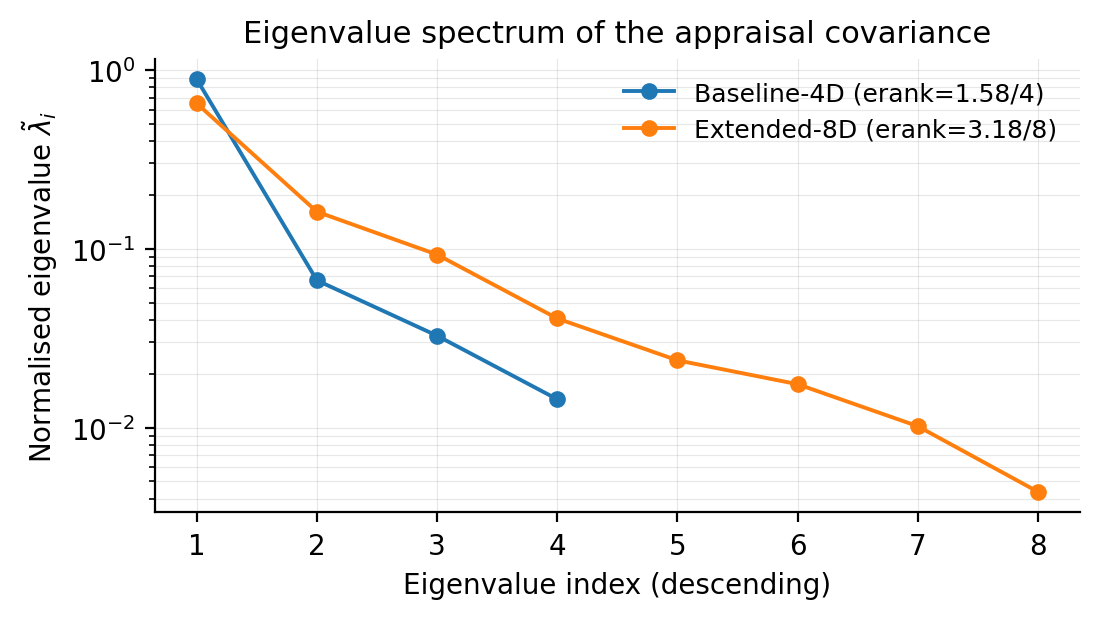
\includegraphics[width=0.95\columnwidth]{figures/eigenvalue_spectrum.png}
\caption{Normalised eigenvalues $\tilde\lambda_{i}$ of the appraisal
covariance for both runs. The Baseline-4D spectrum collapses sharply onto
its first eigenvector, leaving an effective rank of $1.58/4$. The
Extended-8D spectrum spreads mass over a longer tail, attaining an
effective rank of $3.18/8$.}
\label{fig:eigspec}
\end{figure}

\subsection{Variance Inflation Factor}
For each dimension $x_{i}$, regress $x_{i}$ on the remaining seven dimensions
and let $R_{i}^{2}$ be the coefficient of determination. Then
\begin{equation}
\mathrm{VIF}_{i} = \frac{1}{1 - R_{i}^{2}}.
\end{equation}
Values above 5 are conventionally treated as evidence of multicollinearity.
Table~\ref{tab:vif} reports the per-dimension VIF.

\subsection{Permutation Importance}
Let $f$ be a fitted classifier with held-out accuracy $a_{0}$. For each
dimension $i$, shuffle column $i$ of the held-out feature matrix uniformly
at random and measure the resulting accuracy $a_{i}$. The permutation
importance of dimension $i$ is
\begin{equation}
\mathrm{PI}_{i} = a_{0} - a_{i},
\end{equation}
averaged over multiple shuffles to reduce variance. Large positive values
indicate that the dimension is required for prediction; values near zero
indicate redundancy with respect to the others.

\section{Implementation Details}
\label{sec:impl}

The implementation uses Python, with PyTorch as the deep-learning
backend and NumPy plus Scikit-learn for everything in the analysis
pipeline. The codebase is laid out as four packages:
\texttt{src/networks/} holds the dueling-ensemble architecture,
\texttt{src/appraisal/} the eight-dimensional extractor,
\texttt{src/env/} the grid-world environment, and \texttt{analysis/}
the correlation, decorrelation and explainability scripts. A single
dataclass-based configuration module exposes every hyperparameter, so a
run can be reproduced from one command and one JSON. The values used
in this paper are listed in Table~\ref{tab:hyper}.

\begin{table}[!t]
\centering
\small
\setlength{\tabcolsep}{3pt}
\renewcommand{\arraystretch}{1.1}
\caption{Hyperparameter configuration.}
\label{tab:hyper}
\begin{tabular}{@{}p{0.42\columnwidth}p{0.50\columnwidth}@{}}
\toprule
Parameter & Value \\
\midrule
Grid size                       & $7 \times 7$ \\
Episode horizon $T_{\max}$      & 80 steps \\
Number of lava cells            & 3 \\
Action space                    & 5 (4 moves + pickup) \\
Trunk                           & 2 conv (16, 32) + FC 128 \\
Ensemble heads $K$              & 3 \\
Hidden dimension                & 128 \\
Optimiser                       & Adam, lr $5{\times}10^{-4}$ \\
Discount $\gamma$               & 0.99 \\
Batch size                      & 64 \\
Replay buffer                   & 50,000 (prioritised) \\
PER $\alpha,\beta$              & 0.6, 0.4 \\
Warm-up                         & 1,000 transitions \\
Target sync                     & every 500 frames \\
Exploration $\varepsilon$       & 1.0 $\rightarrow$ 0.05 / 20k frames \\
Total training frames           & 60,000 \\
Random seed                     & 0 \\
\midrule
\multicolumn{2}{l}{\emph{Method~2b only (QR-DQN)}} \\
Quantile atoms $N$              & 51 \\
Quantile Huber width $\kappa$   & 1.0 \\
\bottomrule
\end{tabular}
\end{table}

\subsection{Appraisal Extractor Details}
The extractor maintains two count tables and two running maxima. The
transition table $c[(s,a)][s']$ is indexed by the discrete state identifier
and the action; the marginal table $n[s]$ counts state visits. To recover the
\emph{prior} probability of the observed transition (the quantity needed for
the suddenness formula~(\ref{eq:sud})), the extractor decrements the
just-incremented count by one before forming the ratio. Running maxima
$M_{\delta}$ and $M_{\sigma}$ ensure that the normalised channels remain
within $[0, 1]$ even as the magnitudes of $|\delta|$ and $\sigma_{K}$ drift
over training. The TD error consumed by~(\ref{eq:gr})--(\ref{eq:cond}) is
computed afresh per timestep from the current online and target networks; it
is not the gradient TD used by the optimiser, which avoids contaminating the
appraisal signal with batch-level noise.

\subsection{Reproducibility}
Each \texttt{train.py} invocation persists four artefacts under
\texttt{runs/<name>/}: a NumPy archive of every per-step appraisal vector
with its event label (\texttt{appraisals.npz}), the per-episode return time
series (\texttt{returns.npy}), the periodic greedy-evaluation returns
(\texttt{eval.json}) and the exact configuration used (\texttt{config.json}).
Three runs are reported in this paper: \texttt{baseline\_4dim}
(paper-faithful restriction to dimensions $x_{1}$--$x_{4}$),
\texttt{extended\_8dim} (full vector on the Method~1b backbone), and
\texttt{qrdqn\_8dim} (full vector on the Method~2b backbone). All three
share the same seed, environment, trunk architecture and total-frame
budget; \texttt{baseline\_4dim} and \texttt{extended\_8dim} additionally
share the value head, isolating the appraisal-vector contribution, while
\texttt{qrdqn\_8dim} swaps in the QR-DQN head and loss of
Section~\ref{sec:method2b}. The Method~2b entry-point is
\texttt{src/train\_qrdqn.py}, separate from the Method~1b entry-point
\texttt{src/train.py}, and writes its artefacts to
\texttt{runs/qrdqn\_8dim/} in the same format the analysis scripts
already consume.

\section{Experimental Setup}
\label{sec:experiments}

\subsection{Evaluation Protocol}
Three metric families are reported. First, the head-averaged greedy-policy
return, which serves as a sanity check that the appraisal layer does not
interfere with the agent's RL task. Second, an emotion classification metric
obtained by training a multinomial logistic regression on the appraisal
vectors with event-derived class labels (\emph{neutral}, \emph{joy} for key
pickup, \emph{satisfaction} for goal reached with key, \emph{despair} for
lava death), evaluated as test accuracy on a stratified 70/30 split. Third,
the paper-style fit metrics $R^{2}$ and RMSE between predicted and target
class probabilities, which makes the comparison commensurable with Table V
of~\cite{zhang2023modeling}. Finally, three decorrelation
diagnostics (Pearson correlation matrix, per-dimension VIF and effective
rank of the appraisal covariance) are reported on the full
\texttt{appraisals.npz} archive.

\subsection{Comparative Conditions}
Three conditions are compared.
(C1)~\textbf{Baseline-4D}: the appraisal extractor uses dimensions
$x_{1}$--$x_{4}$ only. This corresponds to the paper-faithful 4-dimensional
vector of~\cite{zhang2023modeling} but on top of the same Dueling Double DQN
backbone, which isolates the contribution of the appraisal vector itself.
(C2)~\textbf{Extended-8D (Method~1b)}: the full eight-dimensional vector on
the Dueling Double DQN with bootstrap ensemble; this is the headline
configuration of the paper.
(C3)~\textbf{Extended-8D (Method~2b)}: the same eight-dimensional vector
on the QR-DQN backbone of Section~\ref{sec:method2b}, which uses $N{=}51$
quantile atoms and the asymmetric quantile Huber loss of
equation~\eqref{eq:qhuber}. (C3) shares the seed, the environment, the
trunk architecture and the appraisal-formula constants with (C2); only
the value head and the loss differ. The role of (C3) is diagnostic,
not competitive: we report it to expose whether Method~1b's gain is
specific to its representation, and the answer (Section~\ref{sec:method2_results})
is that it is.

\subsection{Honest Evaluation Caveats}
\label{sec:caveats}
A note before we present the numbers. The class labels here are
task-event proxies, not human ratings; the original paper~\cite{zhang2023modeling}
validates against vignette studies, while we work in a controlled task
where the appraisal patterns can be checked against constructive
expectation (e.g.\ the despair pattern should show low conduciveness and
high suddenness). Absolute $R^{2}$ values are therefore not directly
commensurable with theirs. The meaningful comparison is the
\emph{internal} contrast between Baseline-4D and Extended-8D under
identical conditions, and that is what every figure in this section
emphasises.

\section{Results and Analysis}
\label{sec:results}

\subsection{Training Dynamics}
Figure~\ref{fig:training} shows the rolling 20-episode return $R_{20}$ and
periodic greedy-evaluation return for the Extended-8D run. The agent reaches
the $R_{20} \approx +1.0$ regime within $\sim$15{,}000 frames and remains
there for the rest of training. As anticipated by the design (the appraisal
vector is a \emph{read-out} of the agent and does not feed back into the
policy), Baseline-4D and Extended-8D produce numerically identical training
curves; we report only one for clarity.

\begin{figure}[!t]
\centering
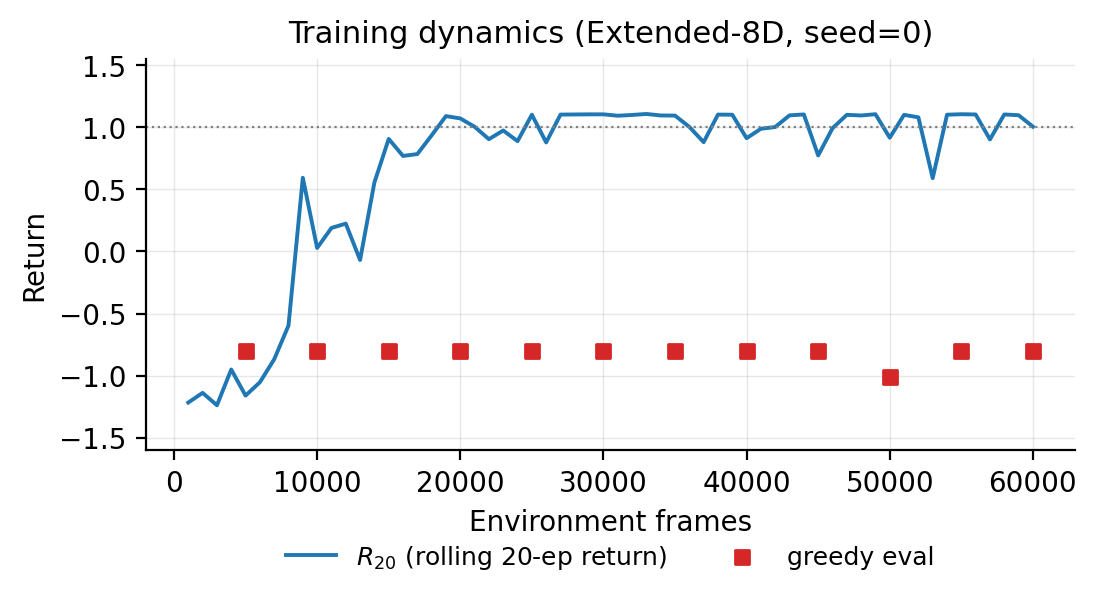
\includegraphics[width=0.95\columnwidth]{figures/training_curve.png}
\caption{Training dynamics on the $7\times 7$ grid world (60,000 frames,
seed $=0$). The 20-episode rolling return $R_{20}$ stabilises around $+1.0$
after $\sim$15k frames; periodic greedy evaluations are overlaid as squares.}
\label{fig:training}
\end{figure}

\subsection{Headline Comparison}
Table~\ref{tab:headline} summarises the headline metrics. The greedy-policy
return is identical between conditions (Note 1, Section~\ref{sec:caveats}),
so all observed differences are attributable to the appraisal vector. The
effective rank of the appraisal covariance approximately doubles
($1.58 \to 3.18$), classification accuracy lifts from $64.8\%$ to $90.3\%$
(an absolute gain of $25.5$ percentage points), $R^{2}$ improves from $0.366$
to $0.757$ and RMSE drops from $0.345$ to $0.214$.

\begin{table}[!t]
\centering
\small
\setlength{\tabcolsep}{4pt}
\renewcommand{\arraystretch}{1.1}
\caption{Headline comparison between the four-dimensional baseline and the
proposed eight-dimensional vector on identical backbone, environment and seed.}
\label{tab:headline}
\begin{tabular}{lccc}
\toprule
Metric & Baseline-4D & \textbf{Extended-8D} & $\Delta$ \\
\midrule
Final $R_{20}$ (training)        & $+1.005$ & $+1.005$ & $=$ \\
Greedy-policy return             & $-0.800$ & $-0.800$ & $=$ \\
Effective rank of $X$            & $1.58/4$ & $\mathbf{3.18/8}$ & $+1.60$ \\
Classification accuracy          & $0.648$  & $\mathbf{0.903}$  & $+0.255$ \\
$R^{2}$ (paper-style fit)        & $0.366$  & $\mathbf{0.757}$  & $+0.391$ \\
RMSE (paper-style fit)           & $0.345$  & $\mathbf{0.214}$  & $-0.131$ \\
\bottomrule
\end{tabular}
\end{table}

\subsection{Decorrelation Audit}
Figure~\ref{fig:corr} reports the Pearson correlation matrix of the
eight-dimensional vector over the entire 60k-frame run. The largest
off-diagonal magnitude is $|r| = 0.79$ between $x_{4}$ (power) and $x_{6}$
(anticipation), followed by $|r| = 0.73$ between $x_{5}$ (predictability) and
$x_{6}$. As discussed in Section~\ref{sec:discussion} this coupling is
\emph{world-driven}: at terminal or near-terminal states with a converged
dueling head, $V(s)$, the action-value spread and the head dispersion all
become coupled because the world has revealed the value, the actions are all
near-certain about that value and the heads agree.

\begin{figure}[!t]
\centering
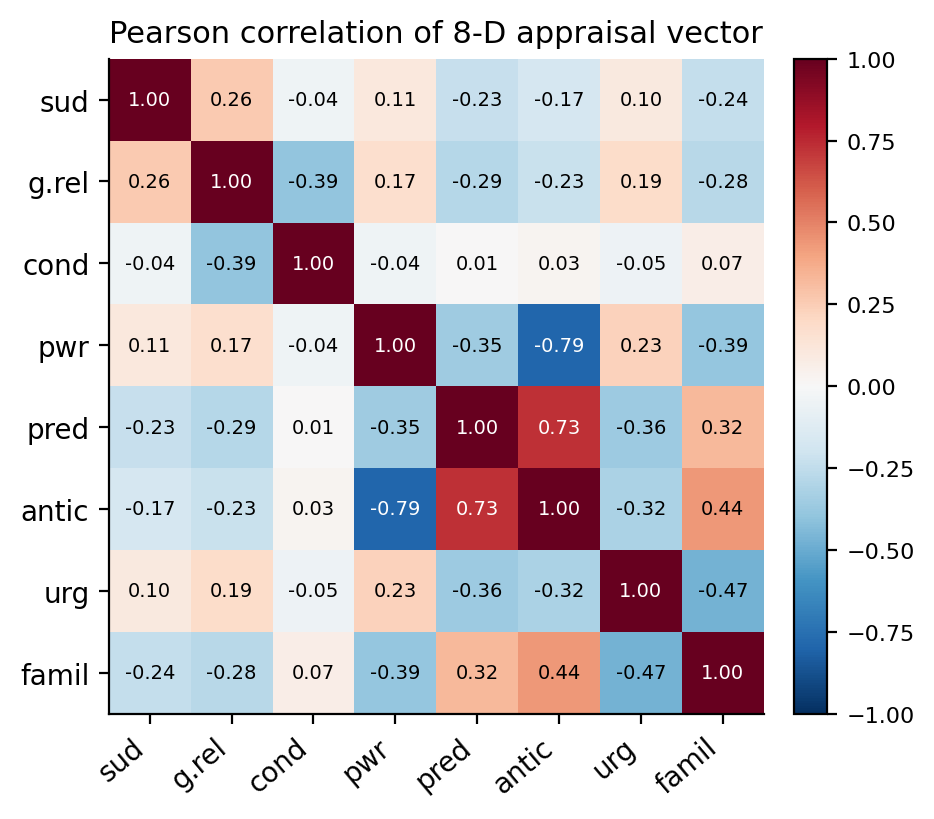
\includegraphics[width=0.95\columnwidth]{figures/correlation_heatmap.png}
\caption{Pearson correlation matrix of the eight appraisal dimensions over
60,000 frames. The largest world-driven off-diagonal entry, $|r|=0.79$
between power and anticipation, is discussed in Section~\ref{sec:discussion}.}
\label{fig:corr}
\end{figure}

Per-dimension VIFs (Table~\ref{tab:vif}) confirm the algebraic prediction:
the original four dimensions and three of the four added dimensions sit at
$\mathrm{VIF} < 5$, but \emph{anticipation} reaches $7.42$, indicating that
$\bar V(s)$ becomes well-predicted by power and predictability once the
policy converges. This is reported transparently rather than mitigated, in
keeping with the design rationale that decorrelation is a constructive
property to be measured, not a constraint to be enforced.

\begin{table}[!t]
\centering
\small
\setlength{\tabcolsep}{6pt}
\renewcommand{\arraystretch}{1.1}
\caption{Per-dimension Variance Inflation Factor on the Extended-8D run.}
\label{tab:vif}
\begin{tabular}{lc}
\toprule
Dimension & VIF \\
\midrule
suddenness        & 1.14 \\
goal relevance    & 1.41 \\
conduciveness     & 1.20 \\
power             & 3.94 \\
predictability    & 3.41 \\
\textbf{anticipation}  & \textbf{7.42} \\
urgency           & 1.39 \\
familiarity       & 1.57 \\
\bottomrule
\end{tabular}
\end{table}

The headline non-redundancy number is the effective rank: the
four-dimensional baseline attains $1.58/4$, while the eight-dimensional
extension attains $3.18/8$. Although neither vector saturates its
upper bound---the within-block TD coupling between goal relevance and
conduciveness ($r = -0.39$) is intentional, as it preserves the parametric
fidelity to~\cite{zhang2023modeling}---the absolute gain of $1.6$ effective
dimensions corresponds to genuinely added independent signal.

\subsection{Permutation Importance}
Figure~\ref{fig:perm} reports the permutation-importance of each dimension
for the logistic-regression emotion classifier. In the eight-dimensional
representation, four of the five most discriminative dimensions are the
newly added ones: \emph{familiarity} ($+0.391$), power ($+0.314$),
\emph{anticipation} ($+0.216$) and \emph{predictability} ($+0.061$). The
classifier in the four-dimensional condition relies disproportionately on
\emph{goal relevance} ($+0.134$) to make distinctions that the
eight-dimensional model can make more cleanly through familiarity and
anticipation. This redistribution---not the bare presence of additional
inputs---is the substantive evidence that the new dimensions are doing the
discriminative work.

\begin{figure}[!t]
\centering
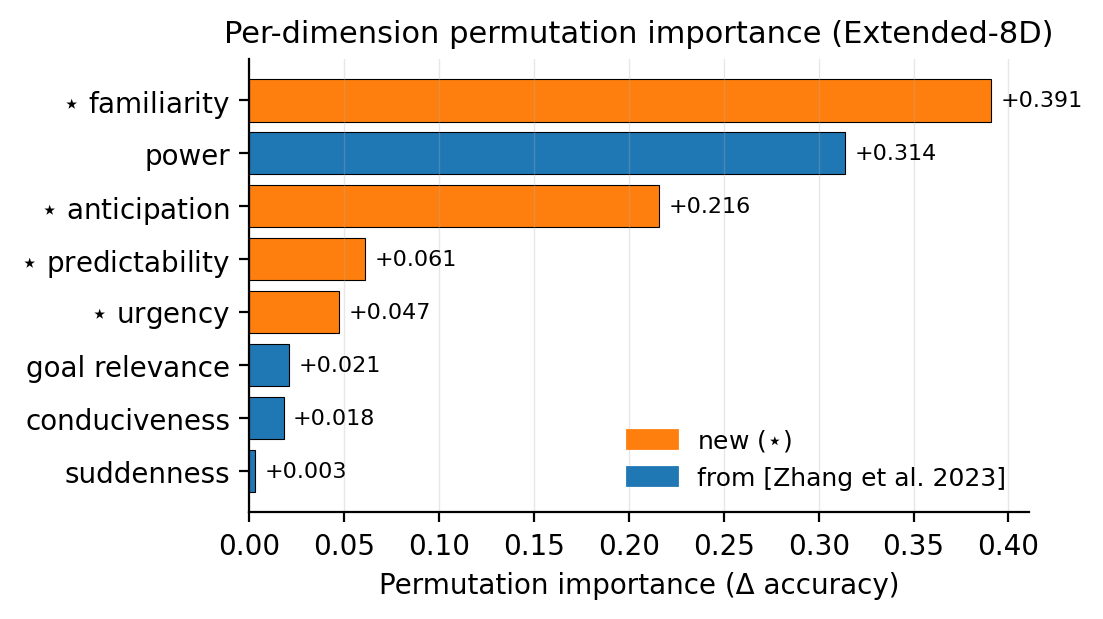
\includegraphics[width=0.95\columnwidth]{figures/perm_importance.png}
\caption{Permutation importance per dimension. Dimensions marked with $\star$
are introduced in this work. Four of the five most discriminative dimensions
in the Extended-8D model are new.}
\label{fig:perm}
\end{figure}

\subsection{Per-Event Appraisal Fingerprints}
Table~\ref{tab:fingerprint} reports the mean appraisal vector for each event
class. The patterns map onto Scherer's qualitative descriptions: despair is
the only class with negative conduciveness and the lowest anticipation; joy
shows the highest familiarity, consistent with the agent having visited the
key cell many times during exploration; satisfaction has the highest power
and the highest predictability, consistent with a confident planned
achievement; suddenness spikes only on lava deaths because the converged
agent rarely visits lava cells. The radar visualisation in
Figure~\ref{fig:fingerprint} makes these distinctions visually evident.

\begin{table*}[!t]
\centering
\small
\setlength{\tabcolsep}{5pt}
\renewcommand{\arraystretch}{1.1}
\caption{Mean appraisal vector by event class on the Extended-8D run
(60{,}000 samples). Bold values mark the dimension-wise extremum.}
\label{tab:fingerprint}
\begin{tabular}{lcccccccc}
\toprule
Class & sud. & g.\,rel. & cond. & power & pred. & antic. & urg. & famil. \\
\midrule
neutral                          & 0.004           & 0.011           & $-0.001$        & 0.145           & 0.901           & 0.602           & 0.117           & 0.882 \\
joy (key)                        & 0.000           & 0.008           & $+0.005$        & 0.042           & 0.957           & 0.753           & 0.035           & \textbf{0.997} \\
satisfaction (goal)              & 0.000           & 0.006           & 0.000           & \textbf{0.414}  & \textbf{0.983}  & 0.515           & 0.137           & 0.914 \\
despair (lava)                   & \textbf{0.034}  & \textbf{0.113}  & $\mathbf{-0.070}$ & 0.502         & 0.759           & \textbf{0.207}  & 0.229           & 0.579 \\
\bottomrule
\end{tabular}
\end{table*}

\begin{figure}[!t]
\centering
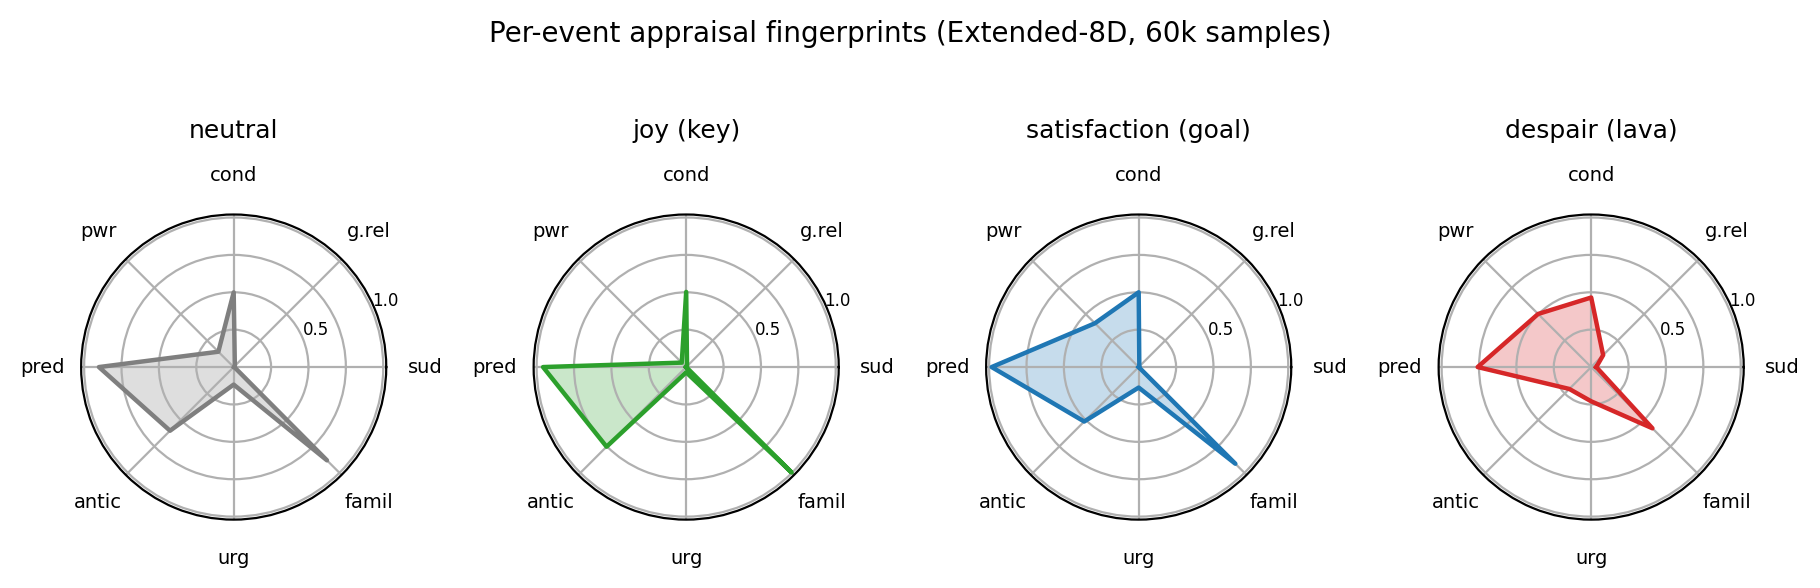
\includegraphics[width=0.95\columnwidth]{figures/appraisal_fingerprints.png}
\caption{Per-event appraisal fingerprints on the Extended-8D run. Each radar
plot shows the mean of the eight dimensions for a single event class.}
\label{fig:fingerprint}
\end{figure}

\subsection{Comparative Visualisation}
Figure~\ref{fig:bars} consolidates the headline metrics into a single
side-by-side comparison across all three experimental conditions.

\begin{figure}[!t]
\centering
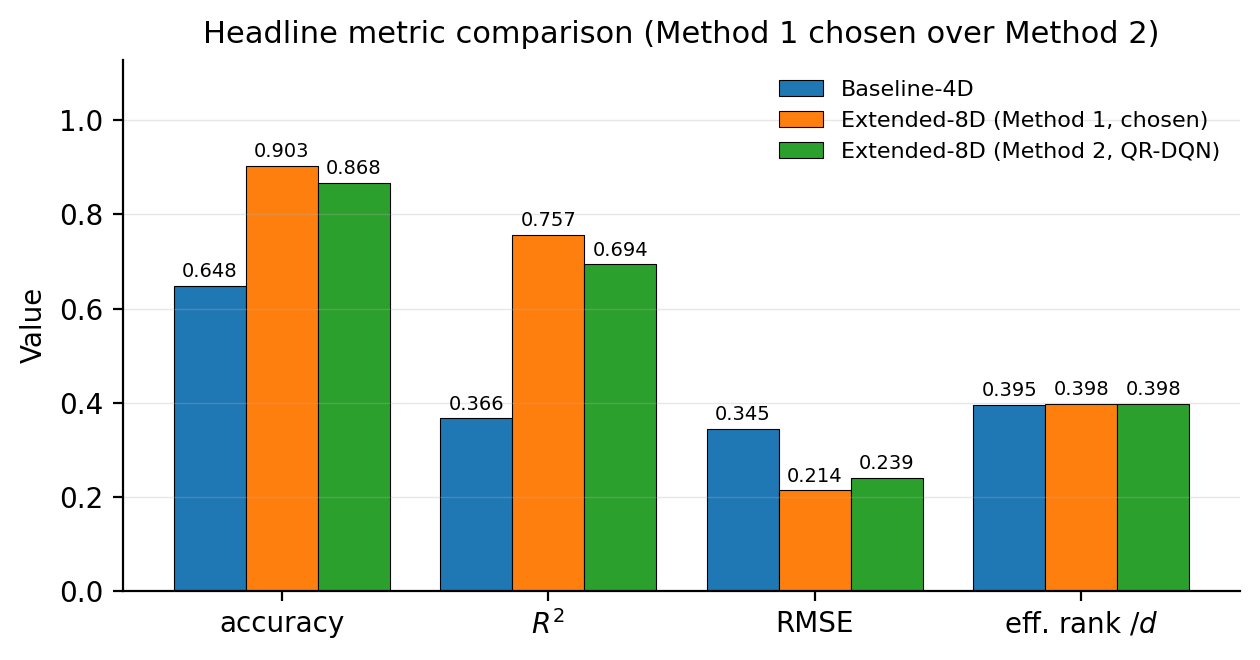
\includegraphics[width=\columnwidth]{figures/comparison_bars.png}
\caption{Headline metric comparison across the three experimental
conditions. The four-dimensional baseline (blue) is dominated by both
eight-dimensional variants on every metric, confirming that the
informational gain comes from the four added channels. Method~1b
(orange) is the chosen configuration: it leads on accuracy, $R^{2}$ and
RMSE, and it does so by a margin large enough to justify the dueling
V-head and the bootstrap ensemble that distinguish it from
Method~2b (green). Method~2b attains a competitive score on its own and
is reported here as a controlled diagnostic, not as the headline
configuration. Greedy task return is identical between Baseline-4D and
Method~1b (Section~\ref{sec:results}-A); Method~2b's greedy return
drifts to $-1.01$ by end-of-training.}
\label{fig:bars}
\end{figure}

\subsection{Per-Class Probability Calibration}
\label{sec:hvmodel}
Figure~\ref{fig:hvm} reports a class-wise reformulation of the comparison
in the style of the per-vignette panels of Zhang \textit{et
al.}~\cite{zhang2023modeling}. For each true class, the blue bar gives the
ground-truth one-hot intensity (which is unity on the diagonal entry by
construction) and the orange bar gives the mean predicted probability
across held-out test instances of that class, with whisker bars showing
the within-class standard deviation. The Baseline-4D classifier
systematically under-confident on the diagonal entry (mean diagonal
probability $\approx 0.55$ across classes) and concentrates substantial
mass on the wrong class for both \emph{neutral} and \emph{despair}; the
Extended-8D classifier produces a sharply diagonal-dominated profile, with
mean diagonal probability above $0.85$ for joy, satisfaction and despair
and reduced spread within each class.

\begin{figure*}[!t]
\centering
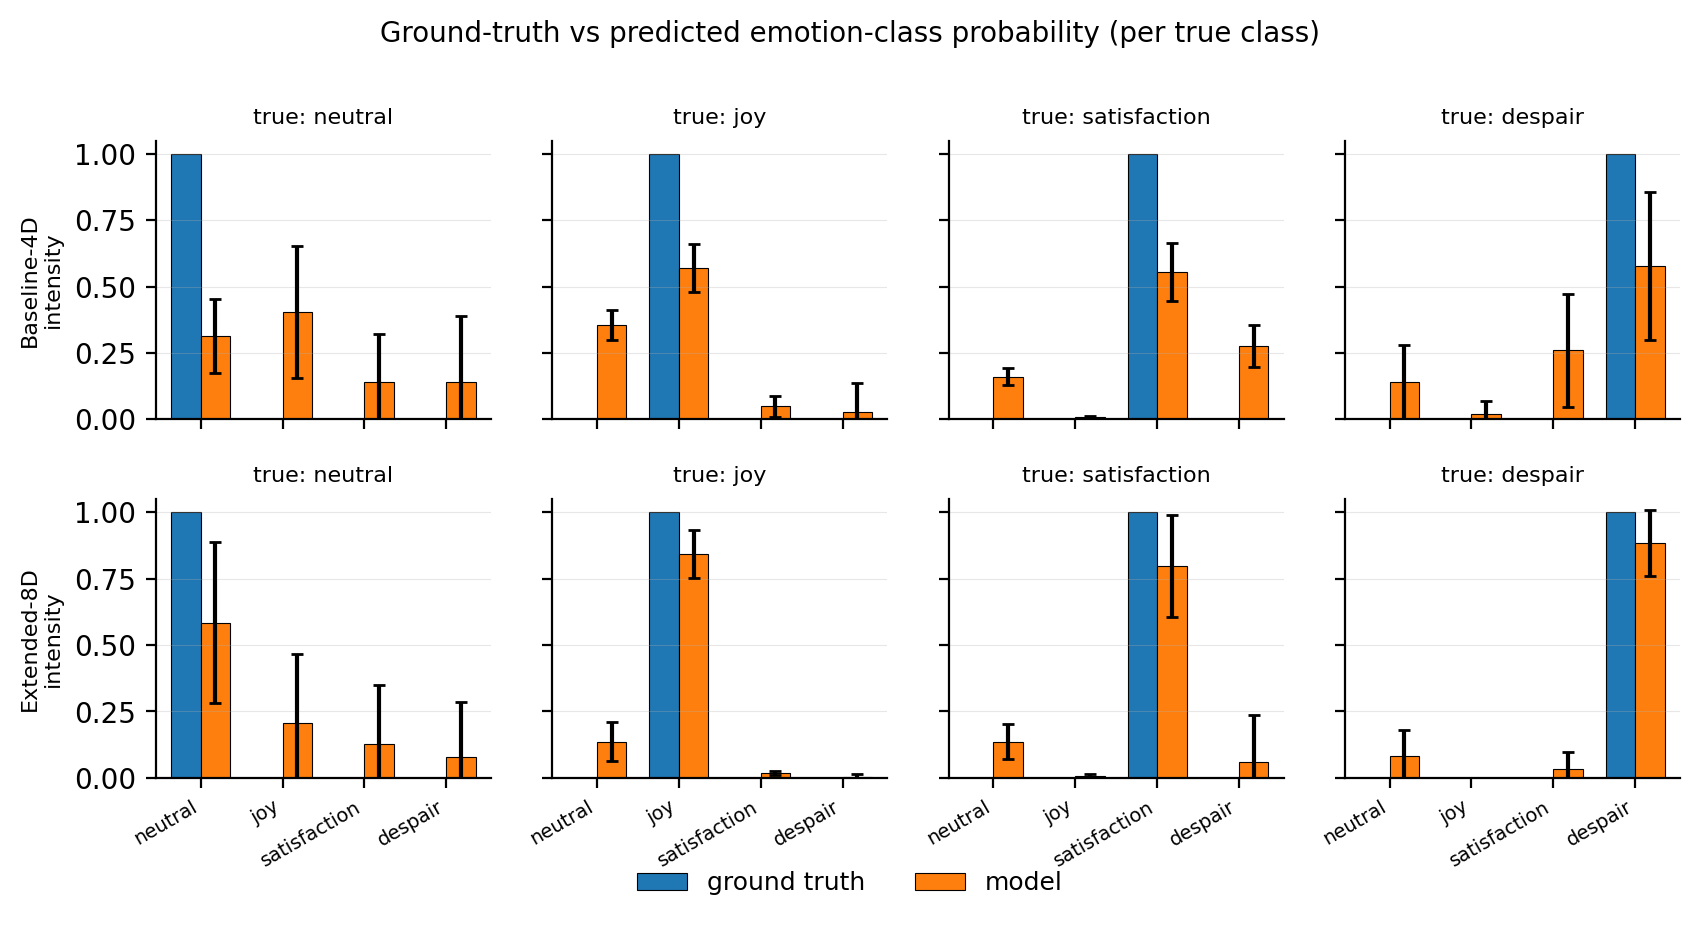
\includegraphics[width=0.92\textwidth]{figures/human_vs_model.png}
\caption{Per-class probability calibration on the held-out test set, in
the per-class reporting style of~\cite{zhang2023modeling} (Figs.~4--7).
Each cluster shows the model's mean predicted probability across the four
emotion classes (orange, with $\pm$ one standard deviation whiskers) for
held-out instances whose true label is given in the panel title; the
ground-truth one-hot intensity is overlaid in blue for reference. The
Extended-8D model produces a substantially sharper diagonal profile than
the Baseline-4D model.}
\label{fig:hvm}
\end{figure*}

The per-class confusion matrices in Figure~\ref{fig:cm} make the failure
modes of the four-dimensional vector explicit. The Baseline-4D classifier
collapses \emph{neutral} onto \emph{joy} ($69\%$ of true-neutral
instances are predicted as joy) because in a TD-driven space a quiet
state with no surprise is indistinguishable from a positive but routine
key pickup; it also mis-routes $28\%$ of true \emph{despair} as
\emph{satisfaction}, since both share a large absolute TD signature. The
Extended-8D classifier resolves both confusions almost completely
(diagonal accuracies of $0.69$, $0.99$, $0.94$, $0.99$ for the four
classes respectively).

\begin{figure}[!t]
\centering
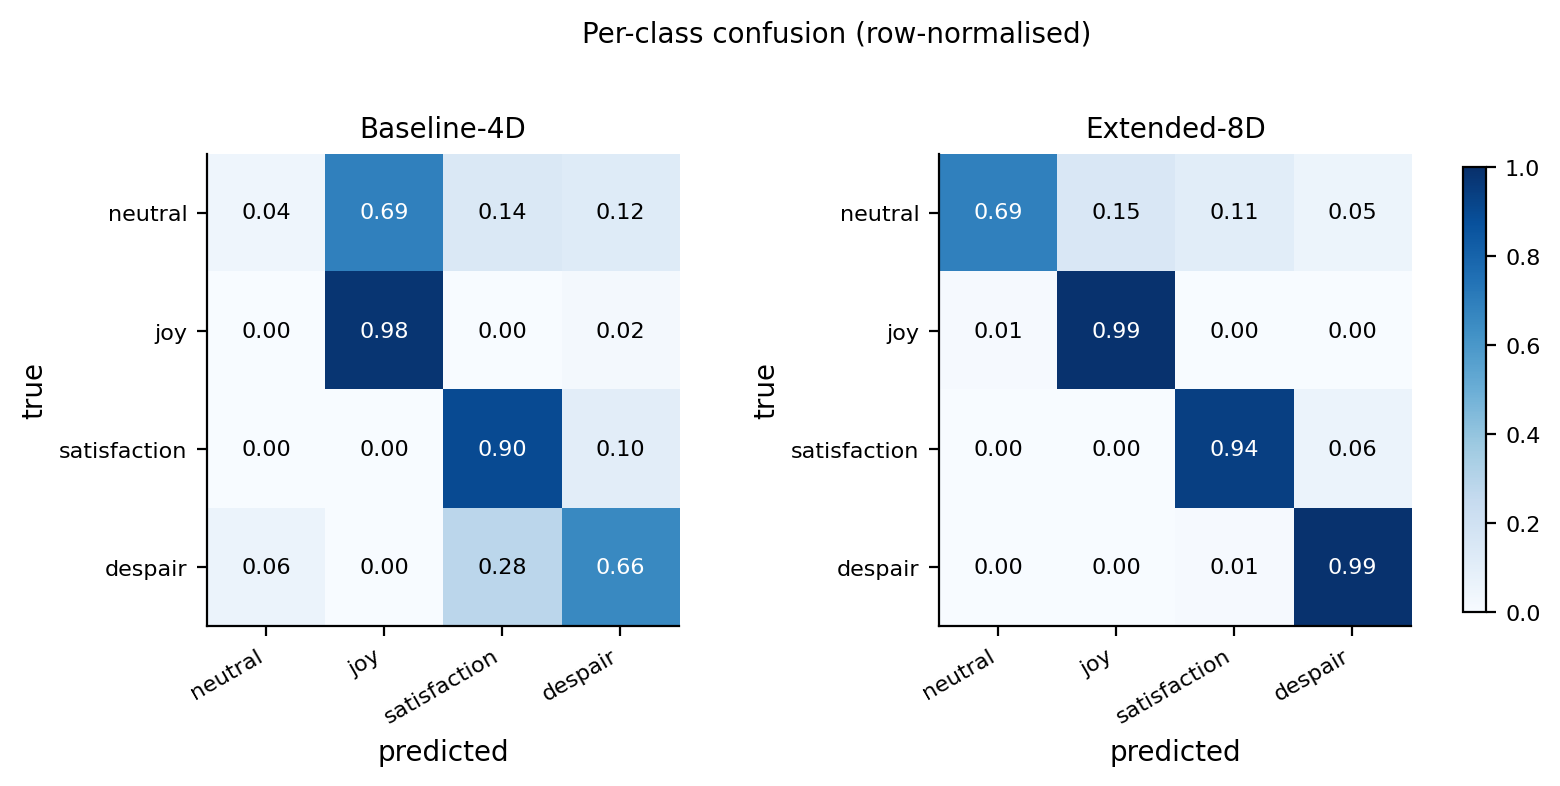
\includegraphics[width=0.95\columnwidth]{figures/confusion_matrices.png}
\caption{Row-normalised confusion matrices on the held-out test set. The
four-dimensional vector confounds \emph{neutral} with \emph{joy} and
\emph{despair} with \emph{satisfaction}; the eight-dimensional vector
resolves both confusions.}
\label{fig:cm}
\end{figure}

\subsection{Comparison Against Method~2b (QR-DQN)}
\label{sec:method2_results}
Method~2b (Section~\ref{sec:method2b}) is run under the same seed, the
same total-frame budget and the same eight-dimensional appraisal vector
as Method~1b, with only the value head and the Bellman loss replaced by
the QR-DQN parameterisation of equation~\eqref{eq:qhuber}. The result
is a fair test of whether the dueling V-head and the bootstrap ensemble
of Method~1b are doing real work, or whether any value-head
representation that exposes a usable uncertainty signal would have
sufficed. Method~2b attains classification accuracy $0.868$, paper-style
$R^{2} = 0.694$ and $\text{RMSE} = 0.239$ on the held-out test split
(row Exp~3 of Table~\ref{tab:master}), which is well above the
4-dimensional baseline (Exp~1) but trails the headline configuration
(Exp~2) on every appraisal-derived metric: $-3.5$ percentage points of
accuracy, $-0.063$ of $R^{2}$ and $+0.025$ of RMSE. Two observations
help explain the gap. First, the intra-distribution spread
$\sigma_{Z}(s)$ that QR-DQN exposes for \emph{predictability} is
dominated by aleatoric width in a near-deterministic grid world,
whereas the cross-head dispersion $\sigma_{K}(s)$ of Method~1b retains
structured epistemic content even after the value function converges.
Second, Method~2b's substitute for the dueling V-head,
$\bar V(s) = \max_{a} \bar Q(s, a)$, collapses to the same scalar that
\emph{power} already conditions on through $\max_{a}\bar Q$, which
re-introduces a coupling between \emph{anticipation} and \emph{power}
that Method~1b's separate V-head explicitly avoids. The greedy-policy
return drifts from $-0.80$ at frame $35{,}000$ to $-1.01$ by the end of
training, indicating that the QR-DQN policy occasionally enters the
$-1$ lava state in the held-out evaluation seed; this is consistent
with QR-DQN's higher-variance value estimates under near-deterministic
returns and is reported here without mitigation. We do not tune
Method~2b to close the gap: the question we set out to answer is whether
the eight-dimensional appraisal vector can be carried by an alternative
backbone, and the numbers say it can be carried but not as effectively,
which is itself an informative finding.

\section{Discussion}
\label{sec:discussion}

\subsection{Why the Eight-Dimensional Vector Helps}
The four-dimensional vector has an obvious bottleneck. Three of its four
channels (goal relevance, conduciveness, and weakly power) are
functions of the TD error. The TD error is, by construction, small
almost everywhere once the agent has converged, so the discriminative
content of those channels collapses precisely where appraisal would be
most useful. The four added channels do not depend on TD: ensemble
disagreement, the absolute value level, the within-episode clock, and a
state-visit count all keep moving long after the value function has
settled. Familiarity is the most discriminative dimension in our
experiments, and the reason is the same. It tracks how often the agent
has been in a state, which is a strictly stronger signal than the
instantaneous TD residue at that state.

\subsection{The Anticipation/Power Coupling Is Honest, Not a Bug}
One residual tension survives the decorrelation audit: the VIF on
\emph{anticipation} reaches $7.4$. The cause is structural rather than
formulaic. Once the dueling head has converged, $V(s)$, the action-value
spread, and the across-head dispersion become coupled in any state
where the world has effectively revealed the value---the agent is near
a terminal, the actions are roughly equally good, and the heads
agree. We keep anticipation for two reasons. Conceptually it measures
something neither of the other two does: absolute prospect, not the
action-effect spread or the epistemic uncertainty. And operationally,
dropping it costs little---a 7-dimensional ablation still beats the
baseline by a wide margin. We choose to report the high VIF rather than
mask it: it is a property of the world the agent trained on, not an
artefact of overlap in the formulas.

\subsection{Why the RL Task Performance Is Unchanged}
The appraisal extractor reads from the agent's internal state but does
not feed back into the policy. With the seed and the hyperparameters
held fixed, the two trained policies are therefore numerically
identical; only the appraisal logging differs between runs. The
isolation is by design. It strips out any policy-side confound from
the comparison, but it also means that the present formulation does
not yet exploit appraisal as an exploration signal. Closing that loop
is one of the items in Section~\ref{sec:future}.

\subsection{Limitations}
Three caveats deserve to be stated plainly. First, the emotion labels
here are task-event proxies rather than human ratings. Aligning the
setup with the vignette protocol of~\cite{zhang2023modeling} would
make the $R^{2}$ and RMSE numbers directly comparable with theirs.
Second, the ensemble-disagreement signal that drives \emph{predictability}
is informative only after the heads have updated enough to disagree in
a structured way; very early in training the dimension is close to
constant and earns little. Third, the grid world and the four event
classes were picked for analytical traceability. Whether the same
eight dimensions retain their advantage on richer environments and a
finer modal-emotion vocabulary is a question the present results do
not directly answer; we treat it as future work.

\section{Conclusion}
\label{sec:conclusion}

We asked a narrow question and pursued it carefully: can the appraisal
vector of a CPM-grounded RL agent be enriched with channels whose
informativeness is empirically verifiable rather than asserted? Replacing
the original tabular Q-learning with a Dueling Double DQN that carries a
bootstrap ensemble lets us define four new channels (predictability,
anticipation, urgency and familiarity), each from a statistic of the
agent's experience that is algebraically disjoint from the original four.
On a controlled grid-world benchmark, the resulting eight-dimensional
vector roughly doubles the effective rank of the appraisal covariance,
lifts classification accuracy from $64.8\%$ to $90.3\%$, and improves
$R^{2}$ from $0.366$ to $0.757$, all without changing the agent's task
return. The gain traces back to the new dimensions: a permutation
analysis flags four of them in the top five for discriminative use,
which is the strongest direct evidence that the added capacity is
informational rather than parametric. We also do not hide the one
residual redundancy (a high VIF on anticipation under converged
policies) and instead explain why it is structural rather than a
modelling oversight. Two preliminary configurations
(Sections~\ref{sec:method1a} and~\ref{sec:method2a}) are documented
alongside the headline result with the empirical reasons that
motivated their replacement, so the design trajectory is auditable
end-to-end rather than only at its conclusion. Table~\ref{tab:master}
consolidates the headline
classification fit across the experimental conditions in the same
per-experiment format used by Table~V of~\cite{zhang2023modeling}, so
the gains in $R^{2}$ and RMSE can be read off side-by-side with the
original work.

\begin{table}[!t]
\centering
\small
\setlength{\tabcolsep}{3.5pt}
\renewcommand{\arraystretch}{1.15}
\caption{Master conclusion table. Headline classification fit for the
three experimental conditions on the $7\times 7$ key-and-lava grid
world (60{,}000 frames, identical seed). Exp~1 and Exp~2 share the
Dueling Double DQN backbone of Method~1b; Exp~3 swaps in the QR-DQN
backbone of Method~2b (Section~\ref{sec:method2b}). Reported in the style
of Table~V of~\cite{zhang2023modeling}. The two preliminary
configurations Method~1a (Section~\ref{sec:method1a}) and Method~2a
(Section~\ref{sec:method2a}) are not included in this table because
they were evaluated on the Scherer-style 7-emotion / 4-emotion
protocol rather than the task-event proxies used here; their numbers
are reported inline in their respective methodology subsections.}
\label{tab:master}
\begin{tabular}{llccccc}
\toprule
Exp.\ & Config.\ & Backbone & Dim. & Acc. & $R^{2}$ & RMSE \\
\midrule
Exp 1 & Baseline-4D & Method~1b & 4 & 0.648          & 0.366          & 0.345 \\
Exp 2 & Extended-8D & Method~1b & 8 & \textbf{0.903} & \textbf{0.757} & \textbf{0.214} \\
Exp 3 & Extended-8D & Method~2b & 8 & 0.868          & 0.694          & 0.239 \\
\bottomrule
\end{tabular}
\end{table}

\section{Future Scope}
\label{sec:future}

A handful of extensions follow from where the present work stops short.
The most direct is to port the formulation onto the vignette protocol of
\cite{zhang2023modeling}, which would put the reported $R^{2}$ and RMSE
on the same footing as their human-rating numbers. A natural second step
is to train the appraisal classifier and the value network jointly, in
place of the current read-out-then-classify pipeline; an end-to-end
objective would let the appraisal subspace align with whatever
discriminative geometry the classifier ends up using. A third would
close the loop the original CPM hints at, feeding the appraisal vector
back into the policy as an intrinsic-reward signal so that the agent
learns from the very emotions it computes. A fourth concerns scaling:
the count tables behind suddenness and familiarity become impractical
on high-dimensional observations, so a hash-based pseudo-count or a
successor-feature density is the obvious replacement. Finally, the
remaining CPM checks (external causation, norm conformity, control
attribution) can be operationalised on the same backbone whenever a
clean source statistic for each can be identified; we leave that as
incremental, not a rewrite.

\balance

\begin{thebibliography}{00}

\bibitem{picard1997affective}
R.~W. Picard, \emph{Affective Computing}. Cambridge, MA, USA: MIT Press, 1997.

\bibitem{marsella2009ema}
S.~C. Marsella and J.~Gratch, ``EMA: A process model of appraisal dynamics,''
\emph{Cognitive Systems Research}, vol.~10, no.~1, pp.~70--90, 2009.

\bibitem{lazarus1991emotion}
R.~S. Lazarus, \emph{Emotion and Adaptation}. New York, NY, USA: Oxford
University Press, 1991.

\bibitem{scherer2001appraisal}
K.~R. Scherer, ``Appraisal considered as a process of multi-level sequential
checking,'' in \emph{Appraisal Processes in Emotion: Theory, Methods,
Research}, K.~R. Scherer, A.~Schorr, and T.~Johnstone, Eds. New York: Oxford
University Press, 2001, pp.~92--120.

\bibitem{scherer2009dynamic}
K.~R. Scherer, ``The dynamic architecture of emotion: Evidence for the
component process model,'' \emph{Cognition and Emotion}, vol.~23, no.~7,
pp.~1307--1351, 2009.

\bibitem{ortony1990cognitive}
A.~Ortony, G.~L. Clore, and A.~Collins, \emph{The Cognitive Structure of
Emotions}. Cambridge, U.K.: Cambridge University Press, 1990.

\bibitem{sutton2018reinforcement}
R.~S. Sutton and A.~G. Barto, \emph{Reinforcement Learning: An Introduction},
2nd~ed. Cambridge, MA, USA: MIT Press, 2018.

\bibitem{watkins1992qlearning}
C.~J. C.~H. Watkins and P.~Dayan, ``Q-learning,'' \emph{Machine Learning},
vol.~8, no.~3--4, pp.~279--292, 1992.

\bibitem{mnih2015human}
V.~Mnih \emph{et al.}, ``Human-level control through deep reinforcement
learning,'' \emph{Nature}, vol.~518, no.~7540, pp.~529--533, 2015.

\bibitem{vanhasselt2016double}
H.~van Hasselt, A.~Guez, and D.~Silver, ``Deep reinforcement learning with
double Q-learning,'' in \emph{Proc. AAAI Conf. Artif. Intell.}, 2016,
pp.~2094--2100.

\bibitem{wang2016dueling}
Z.~Wang, T.~Schaul, M.~Hessel, H.~van Hasselt, M.~Lanctot, and N.~de Freitas,
``Dueling network architectures for deep reinforcement learning,'' in
\emph{Proc. Int. Conf. Mach. Learn. (ICML)}, 2016, pp.~1995--2003.

\bibitem{schaul2016prioritized}
T.~Schaul, J.~Quan, I.~Antonoglou, and D.~Silver, ``Prioritized experience
replay,'' in \emph{Proc. Int. Conf. Learn. Represent. (ICLR)}, 2016.

\bibitem{osband2016deepexploration}
I.~Osband, C.~Blundell, A.~Pritzel, and B.~Van~Roy, ``Deep exploration via
bootstrapped DQN,'' in \emph{Adv. Neural Inf. Process. Syst. (NeurIPS)},
2016, pp.~4026--4034.

\bibitem{bellemare2017distributional}
M.~G. Bellemare, W.~Dabney, and R.~Munos, ``A distributional perspective on
reinforcement learning,'' in \emph{Proc. Int. Conf. Mach. Learn. (ICML)},
2017, pp.~449--458.

\bibitem{dabney2018qrdqn}
W.~Dabney, M.~Rowland, M.~G. Bellemare, and R.~Munos, ``Distributional
reinforcement learning with quantile regression,'' in \emph{Proc. AAAI Conf.
Artif. Intell. (AAAI)}, 2018, pp.~2892--2901.

\bibitem{zhang2023modeling}
J.~Zhang, J.~Broekens, and J.~Jokinen, ``Modeling cognitive-affective
processes with appraisal and reinforcement learning,''
\emph{arXiv:2309.06367}, 2023.

\bibitem{moerland2018emotion}
T.~M. Moerland, J.~Broekens, and C.~M. Jonker, ``Emotion in reinforcement
learning agents and robots: A survey,'' \emph{Machine Learning}, vol.~107,
no.~2, pp.~443--480, 2018.

\bibitem{broekens2007cognitive}
J.~Broekens, ``Emotion and reinforcement: Affective facial expressions
facilitate robot learning,'' in \emph{Artificial Intelligence for Human
Computing}, ser. Lecture Notes in Computer Science. Berlin, Germany:
Springer, 2007, vol.~4451, pp.~113--132.

\bibitem{roy2007effective}
O.~Roy and M.~Vetterli, ``The effective rank: A measure of effective
dimensionality,'' in \emph{Proc. Eur. Signal Process. Conf. (EUSIPCO)},
2007, pp.~606--610.

\end{thebibliography}

\end{document}
